\chapter{Theoretical Study and Methodology}\label{ch:3}

\section{System overview}\label{sec:3.1}

\begin{figure}[htbp]
\centering
\resizebox{\ifdim\width>\linewidth\linewidth\else\width\fi}{!}{% Figure 3.1 of report 45 (system architecture), redrawn in TikZ on a fixed grid: Latin Modern text at \small,
% no overlapping labels, no hyphenation inside the boxes. Dashed arrows = knowledge transferred from EchoNext.
\begin{tikzpicture}[font={\footnotesize\hyphenpenalty=10000\exhyphenpenalty=10000}, >={Stealth[length=2mm]},
  box/.style={draw, rounded corners=2pt, align=center, inner sep=3pt, minimum height=1.2cm, text width=#1},
  box/.default=2.4cm, ar/.style={->, thick}, da/.style={->, thick, dashed}]
\node[box=1.6cm, fill=blue!8]    (pdf)  at (0,0)     {Class-wise folders of ECG printout PDFs (vector)};
\node[box, fill=gray!12]         (ras)  at (3.25,2.3)  {Page raster, text removed, grid filtered};
\node[box, fill=gray!12]         (dig)  at (3.25,0)    {Exact vector digitiser (12$\times$2.5\,s + 10\,s)};
\node[box, fill=gray!12]         (med)  at (3.25,-2.3) {Median beat, fiducials, VCG};
\node[box=2.8cm, fill=green!10]  (cnn)  at (6.85,2.3)  {Pixel CNNs: ResNet, ConvNeXt, EfficientNet};
\node[box=2.8cm, fill=green!10]  (fm)   at (6.85,0)    {ECGFounder, ECG-FM, LSTM, \mbox{1-D} ResNet, MiniRocket};
\node[box=2.8cm, fill=green!10]  (feat) at (6.85,-2.3) {LR, LightGBM, ridge EF on 594 features};
\node[box=3.0cm, fill=blue!8]    (en)   at (6.85,4.4) {EchoNext public data in the printout format (pre-training)};
\node[box=1.9cm, fill=orange!14] (ens)  at (10.45,0)   {Nested ensemble / stacking};
\node[box=1.8cm, fill=orange!14] (dec)  at (13.05,0)   {Decision rule: four classes or triage};
\draw[ar] (pdf.east) -- (dig.west);
\draw[ar] (pdf.north) |- (ras.west);
\draw[ar] (dig.south) -- (med.north);
\draw[ar] (ras.east) -- (cnn.west);
\draw[ar] (dig.east) -- (fm.west);
\draw[ar] (med.east) -- (feat.west);
\draw[ar] (cnn.east) -| (ens.north);
\draw[ar] (fm.east) -- (ens.west);
\draw[ar] (feat.east) -| (ens.south);
\draw[ar] (ens.east) -- (dec.west);
\draw[da] (en.south) -- (cnn.north);
\draw[da] (en.east) -| ($(fm.east)+(0.42,0.38)$) -- ($(fm.east)+(0,0.38)$);
\end{tikzpicture}
}
\caption{System architecture of the Phase I pipeline. Dashed arrows: knowledge transferred from the EchoNext public dataset.}\label{fig:3.1}
\end{figure}

The Phase I pipeline (Figure~\ref{fig:3.1}) has three parts. The printout PDF is digitised exactly, turned into image, signal and feature representations, and passed to the model families. External knowledge enters from the public EchoNext data, redrawn in the hospital printout format.

\section{Dataset}\label{sec:3.2}

\subsection{ECG and echocardiography data collection}\label{sec:3.2.1}

The data come from one tertiary-care hospital and cover 2020--2024: 1,047 ECG printouts of 993 patients, each with an echocardiography report. Every ECG is a standard 12-lead recording stored as a PDF, printed in the usual 3 $\times$ 4 layout (2.5 s per lead) with a 10-s lead II rhythm strip, at 25 mm/s and 10 mm/mV. The LVEF in the echocardiography report is the reference value from which each ECG's class is derived. Name, age, sex and examination date were used to link the ECG and echocardiography records.

\subsection{Spreadsheet loading and cleaning}\label{sec:3.2.2}

The ECG and echocardiography details were kept in separate Excel files, which were read into Python with the Pandas library. Before matching, patient names were normalised (extra spaces, special characters and different name orders removed or unified) so that the same person is written the same way in both files. Only the fields needed later were kept: patient name, age, sex, examination date, ECG file path and LVEF value. Records with missing or unusable entries were flagged so that they could not cause false matches.

\subsection{Patient record matching with fuzzy matching}\label{sec:3.2.3}

Because the same name was not always spelt identically in the two files, exact matching would have missed many pairs. Names were therefore compared with fuzzy string matching (RapidFuzz library), which gives a similarity score and tolerates small spelling differences, swapped word order and spacing. Every candidate pair was then checked against age, sex and examination date, which removed most wrong matches and made the paired dataset more reliable.

\subsection{LVEF extraction and class labels}\label{sec:3.2.4}

For every matched pair the EF value was read from the echocardiography record and converted to a number. Each ECG then received one of the four classes defined in Section~\ref{sec:1.2} (Normal, Mild, Moderate, Severe), and this label was stored with the ECG record for all later steps.

\subsection{Class-wise organisation of the ECG files}\label{sec:3.2.5}

Using the file paths in the matched table, the ECG files were copied into four folders, one per class (Normal, Mild, Moderate, Severe). This structure makes every class easy to access during preprocessing and training.

\subsection{Dataset partitioning}\label{sec:3.2.6}

To keep the evaluation fair, the 1,047 ECGs were split once \emph{by patient}, so that no patient appears in both parts. The \textbf{development set} holds 837 ECGs (384 Normal, 185 Mild, 177 Moderate, 91 Severe) and was used for all modelling. The \textbf{locked test set} holds the other 210 ECGs (96 / 47 / 44 / 23); it was kept apart during development and is not used for any result in this report.

\section{Exact digitisation and the printout renderer}\label{sec:3.3}

The PDFs are vector drawings: each lead is a polyline of about 700 segments, so the trace is recovered exactly. With the row baselines $y_{\text{base}}$ and column origins $ x_{0}$ of the page,
\EqThreeOne
resampled to 500 Hz. The inverse operation, a \emph{printout renderer}, draws any 12-lead signal on a page identical to the hospital's, rounding each point to whole drawing units as the machine does. Redrawn development ECGs match their real pages: 81 \% of drawn points are identical and the read-back error is 5--13 $\mu$ V.

\section{Input representations and features}\label{sec:3.4}

Four representations were built from each printout:

\begin{itemize}
  \item \textbf{page image}: the waveform area with text removed and the grid filtered, for CNNs;
  \item \textbf{aligned signal}: the 12 leads in their own 2.5-s windows on a common 10-s axis, for ECGFounder and the 1-D networks;
  \item \textbf{ECGFounder embeddings}: the 1,024-d final embedding and 150 diagnostic outputs;
  \item \textbf{engineered features}: 594 features, among them 191 clinician-style and vectorcardiographic measurements such as the spatial QRS--T angle, total cosine R-to-T (TCRT) and the QT variability index.
\end{itemize}
\section{Network architectures, preprocessing filters and training}\label{sec:3.5}

\subsection{Preprocessing filters}\label{sec:3.5.1}

\begin{table}[htbp]
\caption{Preprocessing filters and their parameters for each input representation.}\label{tab:3.1}
\small
\begin{tabular}{>{\raggedright\arraybackslash\hspace{0pt}}p{\dimexpr 0.216\linewidth-2\tabcolsep\relax}>{\raggedright\arraybackslash\hspace{0pt}}p{\dimexpr 0.157\linewidth-2\tabcolsep\relax}>{\raggedright\arraybackslash\hspace{0pt}}p{\dimexpr 0.626\linewidth-2\tabcolsep\relax}}
\toprule
\textbf{Input} & \textbf{Step} & \textbf{Filter / operation and parameters} \\
\midrule
Page image (CNNs) & rasterise and crop & vector PDF rendered at 1 px/pt; crop to the waveform area (removes all header text) \\
 & grid removal & colour filter: darkness $=255$ $-$ max$(R, G, B)$ (HSV value); the pink grid has a high value and vanishes \\
 & binarisation & Otsu threshold (clamped) \\
 & denoising & connected components $<6$ px removed (keeps 1-px trace lines that a median filter would erode) \\
 & thickening, resizing & scale-aware dilation; area interpolation to 512 $\times$ 1024, then 256 $\times$ 512 network input \\
 & filter ablations & Gaussian 5 $\times$ 5, $\sigma =1$; median 3 $\times$ 3; bilateral ($ d$ 7, $\sigma$ 50/7); CLAHE (clip 2.0, 8 $\times$ 8 tiles); adaptive Gaussian threshold (block 25, $ C$ 60) \\
\midrule
Digitised signal (ECGFounder) & exact digitisation & vector paths converted at 82 pt/mV and 616$/$3 pt/s; 500 Hz \\
 & power-line notch & IIR notch at 50 Hz, $Q =30$ \\
 & band-pass & 4th-order Butterworth, 0.67--40 Hz, zerophase (forward--backward) \\
 & baseline & 0.4-s moving-median baseline subtracted \\
 & scaling, layout & z-score per lead; 12 leads in their own 2.5-s windows on a 10-s axis (12 $\times$ 5,000) \\
\midrule
\midrule
Engineered features & beat analysis & 0.5 Hz high-pass; R-peak detection; Raligned median beats; vectorcardiogram by the Kors matrix \\
\midrule
EchoNext signals & harmonisation & de-normalisation to $\mu$ V; resampling 250 $\rightarrow$ 500 Hz; cascaded median filters (0.2 s, 0.6 s) for baseline removal; clipping; printout cut (2.5-s windows) \\
\midrule
Pixel CNNs (IMG) & page image & waveform area, text removed, grid filtered; 320 $\times$ 640 (ResNet-18) or 384 $\times$ 768 (ConvNeXt-Tiny, EfficientNet-B2); grey channel repeated to RGB \\
\bottomrule
\end{tabular}
\end{table}


Each representation has its own filter chain (Table~\ref{tab:3.1}): a colour filter removes the pink grid from page images, and a 50 Hz notch, a 0.67--40 Hz band-pass and a moving-median baseline filter clean the signals.

\subsection{Network layers and activation functions}\label{sec:3.5.2}

Table~\ref{tab:3.2} gives the layers, kernels, activation functions, normalisation and size of every network. The activation functions used are
\EqThreeTwo
where $\Phi$ is the standard normal distribution function. Every four-class network ends in a softmax, and ordinal heads use sigmoids for $ P(y> k)$.

\subsection{Training settings and training accuracy}\label{sec:3.5.3}

Every model in this report was trained until its training accuracy reached (nearly) 100 \%, for as many epochs or iterations as it needed; the settings of every model family are listed in Table~\ref{tab:3.6}. Image CNNs and the 1-D SE-ResNet were trained with AdamW (learning rate 10$^{-3}$ after a short warm-up, then constant), batch 16 and class-weighted cross-entropy, without augmentation, label smoothing, weight averaging, weight decay or early stopping, until their training accuracy reached at least 99.5 \%; no network needed its epoch cap. ECGFounder was fine-tuned in the same way with differential learning rates (backbone 10$^{-4}$, head 10$^{-3}$). The MLP heads were trained without weight decay or early stopping until they reached 100 \% (at most 3,000 epochs), the linear and logistic models with almost no regularisation (C = 10,000 or L2 10$^{-6}$), and gradient boosting with 2,000 trees, one sample per leaf allowed and no shrinkage penalty. Table~\ref{tab:3.3} compares training and validation accuracy, and Table~\ref{tab:3.5} shows how the twelve main models are built.

\begin{itemize}
  \item \textbf{Image and signal networks} reach 0.996--1.000 training accuracy in 12--57 epochs, but 0.35--0.56 on the 168 validation ECGs. Their training loss falls below 0.04 while the validation loss rises to 1.7--6.4 (Figure~\ref{fig:3.2}): they memorise the training ECGs, and every CNN reached its highest validation accuracy before its last epoch.
  \item \textbf{Foundation-feature heads} reach 1.000 on the training folds against 0.49--0.54 held out. ECGFounder fine-tuning reaches 0.996 in 12 epochs and gives the best validation accuracy of the fixed split (0.560). A logistic regression on header and clinical features stops at 0.589 even without regularisation, because straight-line class boundaries cannot separate every training ECG.
  \item With 837 ECGs for 30.7 million ECGFounder parameters, frozen features, nested selection and ensembling were used in all later phases.
\end{itemize}
\subsection{Analysis of transfer learning}\label{sec:3.5.4}

\begin{table}[htbp]
\caption{Layers, activation functions, normalisation and size of every network in this report.}\label{tab:3.2}
\footnotesize\setlength{\tabcolsep}{4pt}
\begin{tabular}{>{\raggedright\arraybackslash\hspace{0pt}}p{\dimexpr 0.172\linewidth-2\tabcolsep\relax}>{\raggedright\arraybackslash\hspace{0pt}}p{\dimexpr 0.420\linewidth-2\tabcolsep\relax}>{\raggedright\arraybackslash\hspace{0pt}}p{\dimexpr 0.131\linewidth-2\tabcolsep\relax}>{\raggedright\arraybackslash\hspace{0pt}}p{\dimexpr 0.155\linewidth-2\tabcolsep\relax}>{\raggedright\arraybackslash\hspace{0pt}}p{\dimexpr 0.119\linewidth-2\tabcolsep\relax}}
\toprule
\textbf{Network} & \textbf{Layers and blocks} & \textbf{Activation} & \textbf{Norm.} & \textbf{Params} \\
\midrule
ResNet-18 & 7 $\times$ 7 conv stem + max-pool; 4 stages $\times$ 2 basic blocks of two 3 $\times$ 3 convs (64--512 channels); global average pool; FC(4) --- 18 weight layers & ReLU & BatchNorm & 11.2 M \\
ECGNet (custom) & 7 $\times$ 7/2 stem; 4 stages of 1--1--2--2 residual SE blocks (widths 64--256) with time-elongated 3 $\times$ 5 kernels; [GAP $\|$ GMP]; dropout 0.3; FC(4) ---13 conv layers & ReLU; sigmoid (SE) & BatchNorm & 6.3 M \\
EfficientNet-B0 & 3 $\times$ 3 stem; 16 MBConv blocks in 7 stages with SE; 1 $\times$ 1 head conv; FC(4) & SiLU & BatchNorm & 4.0 M \\
MobileNetV3-Large & 3 $\times$ 3 stem; 15 inverted-residual bottlenecks, SE in 8; 1 $\times$ 1 head & h-swish, ReLU & BatchNorm & 4.2 M \\
ConvNeXt-Atto & 4 $\times$ 4 patchify stem; 4 stages of 2--2--6--2 blocks (7 $\times$ 7 depth-wise conv + MLP) & GELU & LayerNorm & 3.4 M \\
1-D SE-ResNet & 1-D residual blocks, kernel 9, SE; [GAP $\|$ GMP]; FC(4) & ReLU & BatchNorm & 4.5 M \\
ECGFounder (Net1D) & 1-D conv stem (kernel 16, stride 2); 7 stages of 2--2--2--3--3--4--4 blocks (20 blocks; 64--1,024 filters), grouped kernel-16 convs with SE; GAP $\rightarrow$ 1,024-d embedding & Swish & none & 30.7 M \\
MLP head / fusion & dropout 0.5 $\rightarrow$ linear 64 $\rightarrow$ GELU $\rightarrow$ dropout 0.5 $\rightarrow$ linear 4 & GELU & standardised input & 66 k \\
Meta-learners & multinomial logistic regression; Frank--Hall ordinal (3 binary logistic models) & softmax; sigmoid & standardised & $<1$ k \\
\bottomrule
\end{tabular}
\end{table}


\begin{table}[htbp]
\caption{Training against validation accuracy of the main networks, every network trained until its training accuracy reached (nearly) 100 \% (no early stopping, augmentation, weight decay, label smoothing or weight averaging). Training accuracy is measured on all training ECGs in evaluation mode. Sorted by training accuracy within each part. Epochs: until the target was reached (CNNs $\ge$ 99.5 \%); solver / iter. = models not trained in epochs.}\label{tab:3.3}
\footnotesize\setlength{\tabcolsep}{3pt}
\begin{tabular}{>{\raggedright\arraybackslash\hspace{0pt}}p{\dimexpr 0.420\linewidth-2\tabcolsep\relax}>{\raggedright\arraybackslash\hspace{0pt}}p{\dimexpr 0.120\linewidth-2\tabcolsep\relax}>{\raggedright\arraybackslash\hspace{0pt}}p{\dimexpr 0.130\linewidth-2\tabcolsep\relax}>{\raggedright\arraybackslash\hspace{0pt}}p{\dimexpr 0.150\linewidth-2\tabcolsep\relax}>{\raggedright\arraybackslash\hspace{0pt}}p{\dimexpr 0.180\linewidth-2\tabcolsep\relax}}
\toprule
\textbf{Network} & \textbf{Epochs} & \textbf{Training accuracy} & \textbf{Validation / held-out accuracy} & \textbf{Train / val loss} \\
\midrule
\multicolumn{5}{>{\raggedright\arraybackslash\hspace{0pt}}p{\dimexpr\linewidth-2\tabcolsep\relax}}{\textit{Networks of the initial project and Phase 1, fixed split (669 training / 168 validation ECGs)}} \\
EfficientNet-B0 & 37 & 1.000 & 0.417 & 0.002 / 5.230 \\
1-D SE-ResNet & 32 & 0.999 & 0.435 & 0.014 / 3.005 \\
ECGNet & 21 & 0.999 & 0.435 & 0.005 / 3.354 \\
MobileNetV3-Large & 57 & 0.999 & 0.387 & 0.003 / 5.845 \\
ResNet-18 & 24 & 0.997 & 0.423 & 0.010 / 2.702 \\
ECGFounder fine-tuned (stages 5--6) & 12 & 0.996 & 0.560 & 0.036 / 1.657 \\
ConvNeXt-Atto & 53 & 0.996 & 0.345 & 0.025 / 6.426 \\
\multicolumn{5}{>{\raggedright\arraybackslash\hspace{0pt}}p{\dimexpr\linewidth-2\tabcolsep\relax}}{\textit{Frozen-feature heads, development cross-validation (mean of the 15 folds)}} \\
FUSION-MLP (header + ECGFounder, MLP head) & 112 & 1.000 & 0.538 & -- \\
ECGF-MLP (ECGFounder + MLP head) & 108 & 1.000 & 0.536 & -- \\
ECGF-linear (ECGFounder + linear head) & 100 iter. & 1.000 & 0.491 & -- \\
HDRCLIN-LR (header + clinical features, logistic regression) & solver & 0.589 & 0.486 & -- \\
\bottomrule
\end{tabular}
\end{table}


\begin{figure}[htbp]
\centering
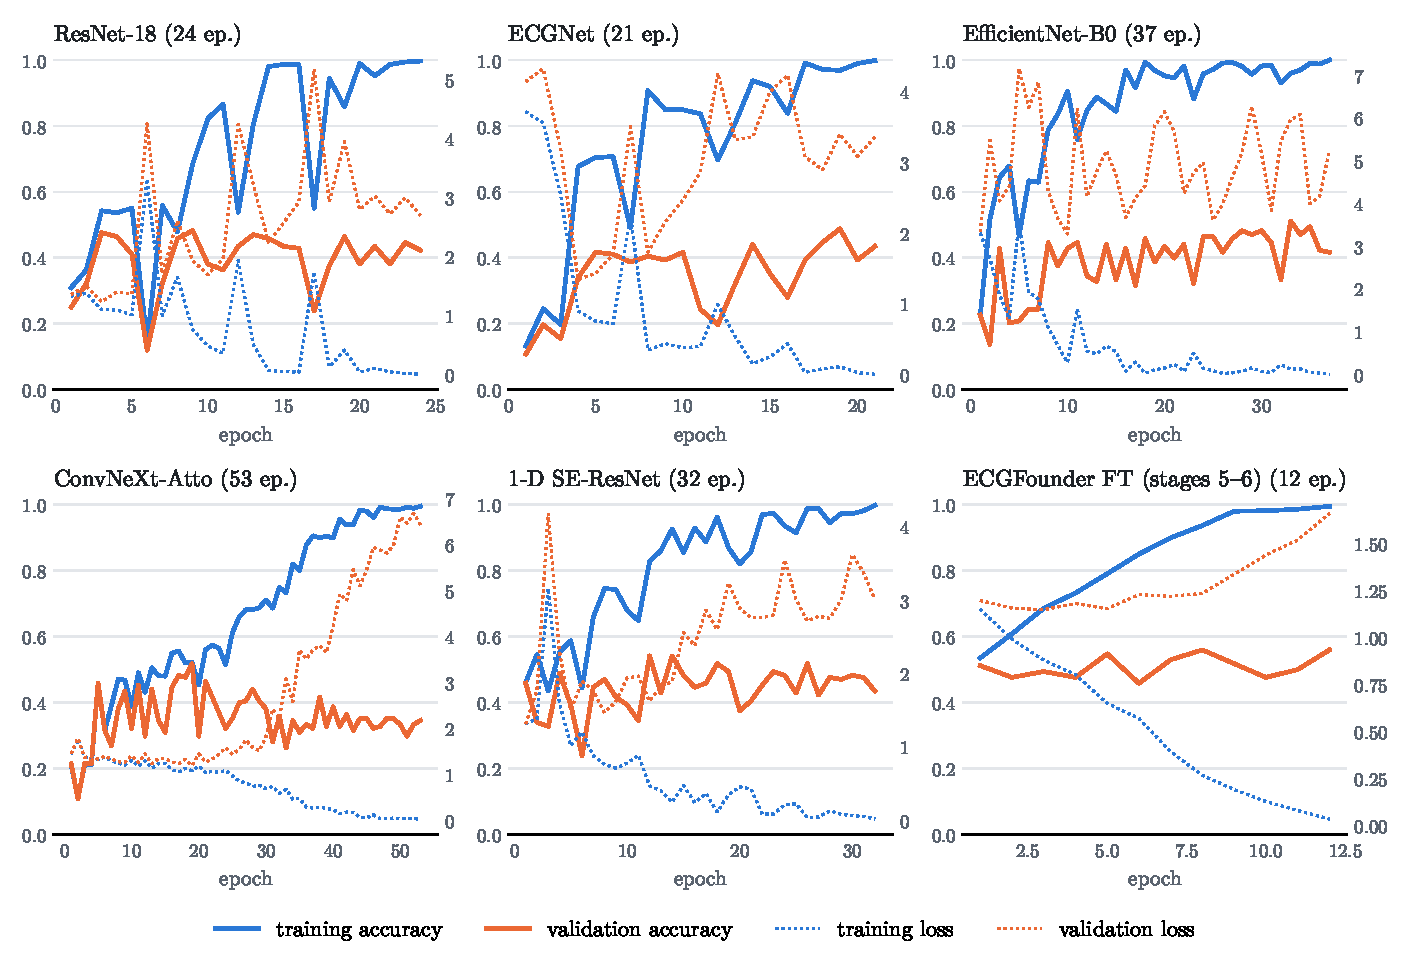
\includegraphics[width=1.00\linewidth,height=0.80\textheight,keepaspectratio]{figures/fig_3_2}
\caption{Training curves of six representative networks trained until their training accuracy reached $\ge$ 99.5 \%: training and validation accuracy (solid) and loss (dotted) per epoch, fixed split.}\label{fig:3.2}
\end{figure}

\begin{table}[htbp]
\caption{Transfer learning: source, how the knowledge was transferred and what it gave on the hospital printouts (every model trained to (nearly) 100 \% training accuracy).}\label{tab:3.4}
\small
\begin{tabular}{>{\raggedright\arraybackslash\hspace{0pt}}p{\dimexpr 0.199\linewidth-2\tabcolsep\relax}>{\raggedright\arraybackslash\hspace{0pt}}p{\dimexpr 0.295\linewidth-2\tabcolsep\relax}>{\raggedright\arraybackslash\hspace{0pt}}p{\dimexpr 0.505\linewidth-2\tabcolsep\relax}}
\toprule
\textbf{Source} & \textbf{Transfer method} & \textbf{Result on the hospital data} \\
\midrule
ImageNet (1.3 M natural images) & initialise ResNet-18; train on the hospital page images & 0.997 training, 0.423 validation (fixed split; best 0.482 before the last epoch): natural-image features transfer only partly to thin line drawings \\
ECGFounder (10.8 M ECGs, 150 labels) & frozen 1,024-d embedding + linear or MLP head & 1.000 training, 0.491--0.536 held out (CV); EF regression $r$ 0.624; the backbone of every main model \\
 & partial fine-tuning (stages 5--6) & 0.996 training, 0.560 validation (fixed split): the best network on that split \\
EchoNext signals (4,827 US ECG--echo pairs) & models trained only on EchoNext; only their decision thresholds tuned on hospital data & 0.78--1.00 training and 0.46--0.76 validation accuracy on EchoNext; 0.41--0.54 four-class accuracy on the hospital ECGs \\
 & EchoNext models as ensemble members & SUPER ensembles 0.548--0.558, the best all-patient results; 0.539 for the same recipe without them \\
EchoNext images (drawn as printouts) & pixel CNN trained on the printout images & 0.999 training, 0.725 validation on EchoNext; 0.505 on the hospital pages \\
\bottomrule
\end{tabular}
\end{table}


\begin{table}[htbp]
\caption{How the twelve main models are built, sorted by training accuracy. ECGFounder (Net1D; 61 convolution and 40 linear layers in 7 stages of 20 residual blocks; 30.7 M parameters) was pre-trained on 10.8 million ECGs and is kept frozen, so only the heads are trained on the hospital ECGs. Epochs: median over the 15 folds to reach 100 \% training accuracy; $^{b}$ epochs of the member FUSION-MLP; $^{c}$ epochs of the member ECGF-MLP.}\label{tab:3.5}
\footnotesize\setlength{\tabcolsep}{3pt}
\begin{tabular}{>{\raggedright\arraybackslash\hspace{0pt}}p{\dimexpr 0.140\linewidth-2\tabcolsep\relax}>{\raggedright\arraybackslash\hspace{0pt}}p{\dimexpr 0.200\linewidth-2\tabcolsep\relax}>{\raggedright\arraybackslash\hspace{0pt}}p{\dimexpr 0.300\linewidth-2\tabcolsep\relax}>{\raggedright\arraybackslash\hspace{0pt}}p{\dimexpr 0.120\linewidth-2\tabcolsep\relax}>{\raggedright\arraybackslash\hspace{0pt}}p{\dimexpr 0.120\linewidth-2\tabcolsep\relax}>{\raggedright\arraybackslash\hspace{0pt}}p{\dimexpr 0.120\linewidth-2\tabcolsep\relax}}
\toprule
\textbf{Model} & \textbf{Inputs} & \textbf{Layers / structure} & \textbf{Params} & \textbf{Epochs} & \textbf{Training acc.} \\
\midrule
Triage$^{\dagger}$ & ECGFounder + 118 clinician features $\rightarrow$ EF; IMG-C3 & ridge + LightGBM EF regressors $\rightarrow$ EF grade (3 cut-points) + margin; answers when the grade agrees with IMG-C3 & regressors + 4 & 4,000 trees & 1.000 \\
LGBM-FEAT & 16 header + 403 engineered waveform features (419) & 2,000 boosting rounds $\times$ 4 classes, 31 leaves per tree & 8,000 trees & 2,000 trees & 1.000 \\
FUSION-MLP & 16 header + ECGFounder embedding (1,040) & MLP head as ECGF-MLP; 3 seeds & 67.0 k trained & 112 & 1.000 \\
ECGF-MLP & frozen ECGFounder embedding (1,024) & frozen backbone + MLP: dropout, linear 1,024 $\rightarrow$ 64, GELU, dropout, linear 64 $\rightarrow$ 4; 3 seeds & 65.9 k trained & 108 & 1.000 \\
IMG-C3 & IMG-vote & IMG-vote + nested prior rule & members + 1 & 108$^{c}$ & 1.000 \\
C1 & FUSION-MLP + ECGF-linear + HDRCLIN-LR & average of the 3 members' probabilities & members & 112$^{b}$ & 1.000 \\
IMG-vote & ECGF-MLP + ECGF-linear (image only) & average of the 2 members' probabilities & members & 108$^{c}$ & 1.000 \\
ECGF-linear & frozen ECGFounder embedding (1,024) & frozen backbone + 1 linear layer (1,024 $\rightarrow$ 4) & 4.1 k trained & 100 iter. & 1.000 \\
C3 & C1 & C1 + nested prior rule (one $\alpha$ chosen on inner out-of-fold predictions) & members + 1 & 112$^{b}$ & 0.995 \\
CLIN-LR & 118 image-only clinician features & 1 linear layer (118 $\rightarrow$ 4) & 476 & solver & 0.720 \\
HDRCLIN-LR & 16 header + 28 clinical ECG features (44) & 1 linear layer (44 $\rightarrow$ 4) & 180 & solver & 0.589 \\
HDR-LR & 16 header measurements (age, sex, rate, intervals, axes) & 1 linear layer (16 $\rightarrow$ 4) & 68 & solver & 0.529 \\
\bottomrule
\end{tabular}
\end{table}


\begin{table}[htbp]
\caption{Training settings of every model family. Inputs, labels, architectures, folds and decision rules are those of each stage; every model was trained for as many epochs or iterations as it needed, until its training accuracy reached (nearly) 100 \%.}\label{tab:3.6}
\small
\begin{tabular}{>{\raggedright\arraybackslash\hspace{0pt}}p{\dimexpr 0.360\linewidth-2\tabcolsep\relax}>{\raggedright\arraybackslash\hspace{0pt}}p{\dimexpr 0.640\linewidth-2\tabcolsep\relax}}
\toprule
\textbf{Model family} & \textbf{Training} \\
\midrule
MLP heads and fusion networks & AdamW, weight decay 0, no early stopping; until 100 \% training accuracy (at most 3,000 epochs) \\
Linear and logistic models & almost no regularisation (L2 $10^{-6}$ or C = 10,000), solved to convergence \\
Gradient boosting & 2,000 trees (4,000 for the EF regressor), one sample per leaf allowed, L2 0, no early stopping \\
Image CNNs, 1-D SE-ResNet, ECGFounder fine-tuning & AdamW, constant learning rate after a short warm-up; no augmentation, label smoothing, weight averaging or weight decay; until training accuracy $\ge$ 99.5 \% (epoch caps 100 / 150 / 60, never reached) \\
$k$-nearest neighbours & $k$ = 15, distance weighting \\
Ensembles, stacks, decision rules & built from the members above; weights, thresholds and prior rules chosen on inner out-of-fold predictions; meta-learners C = 10,000 \\
\bottomrule
\end{tabular}
\end{table}


Transfer learning was used in four forms, from natural images to EF-labelled ECGs (Table~\ref{tab:3.4}). The closer the source is to the target, the larger the gain. On the same fixed split, ECG pre-training (ECGFounder fine-tuned, 0.560) beat ImageNet pre-training (ResNet-18, 0.423) by 13.7 points, and EF-labelled public ECGs (EchoNext) supplied the members behind the best all-patient ensembles: the best ensemble reaches 0.558 with its EchoNext members and 0.539 without them. Models trained only on US patients reach up to 0.539 four-class accuracy on our printouts with only their decision thresholds tuned on hospital data, which also validates the printout conversion, and a pixel CNN trained only on EchoNext ECGs drawn as hospital printouts reaches 0.505 on the hospital pages.

\section{Evaluation protocol}\label{sec:3.6}

\begin{itemize}
  \item \textbf{Cross-validation:} patient-grouped 5-fold CV repeated three times (15 cells), identical folds for every model.
  \item \textbf{Nested choices:} every hyper-parameter, class weight, threshold and ensemble member is chosen inside the training folds \cite{ref37}. Class weights maximise accuracy subject to every recall $\ge0.18$ (fallback 0.15):
\EqThreeThree
  \item \textbf{Intervals and tests:} corrected resampled $t$ statistic \cite{ref38} with Holm adjustment \cite{ref39}:
\EqThreeFour
  \item \textbf{Integrity:} every study, including the training to 100 \%, was pre-registered in a dated document before it was run; the locked test set is not used in this report.
\end{itemize}
